\documentclass[border=4pt]{standalone}
\usepackage{pgfplots}
\pgfplotsset{compat=1.18}

\begin{document}
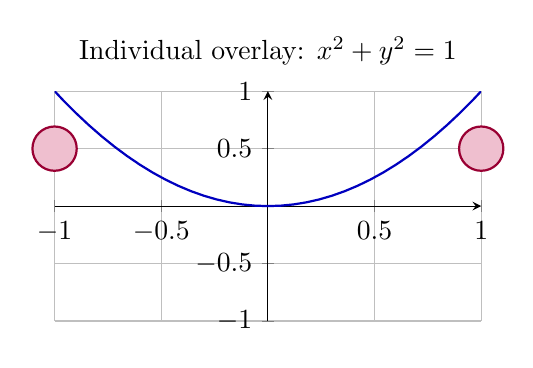
\begin{tikzpicture}
  \begin{axis}[
    width=7cm,
    height=4.5cm,
    xmin=-1, xmax=1,
    ymin=-1, ymax=1,
    enlargelimits=false,
    clip mode=individual,
    axis lines=middle,
    grid=major,
    title={Individual overlay: $x^2+y^2=1$}
  ]
    \addplot[domain=-1.2:1.2,samples=41,blue!75!black,thick] {x*x};
    \filldraw[purple!80!black,fill=purple!25,thick] (axis cs:-1,0.5) circle (8pt);
    \filldraw[purple!80!black,fill=purple!25,thick] (axis cs:1,0.5) circle (8pt);
  \end{axis}
\end{tikzpicture}
\end{document}
